
A world is easily divided into different aspects. There are the sky, the oceans and the land. The land contain different terrain, with different types of ground and vegetation. There is a sun orbiting the world, casting rays of light and in the process creating reflections and indirectly making shadows.\\
\\
A procedural world is generated by carefully chosen algorithms. Our world is procedurally generated anew in a new unique constellation on every run, or a seed can be provided to generate specific worlds. The terrain is first formed, then the ground texturing and the vegetation, both dependent on properties of the terrain. The shadows depend on the sun and the waves on the terrain as well as on time itself.

\subsection{Sky}
The sky is achieved using a high-resolution texture of a sky mapped to a skybox. The mathematical location of the sun is placed as close as possible to the sun appearing in this texture. This gives shadows and shading a natural feel. The texture has been manually modified at the horizon to fade towards a shadowish gray color. The color is the same as the one objects are distance-fogged with. This makes the sky melt into the ocean in a very nice way. 

\subsection{Ocean}
The water is made up of a normal-mapped square and a blue color. The normal map is repeated over the square and is moving in texture space, giving the illusion of a wind. The normal map movement cycles such that when the water normal map has been totally displaced, it starts over again from its original position. This movement makes the water glitter from a far, see figure \ref{fig:water}.
\begin{figure}[H]
\begin{subfigure}{.5\textwidth}
  \centering
  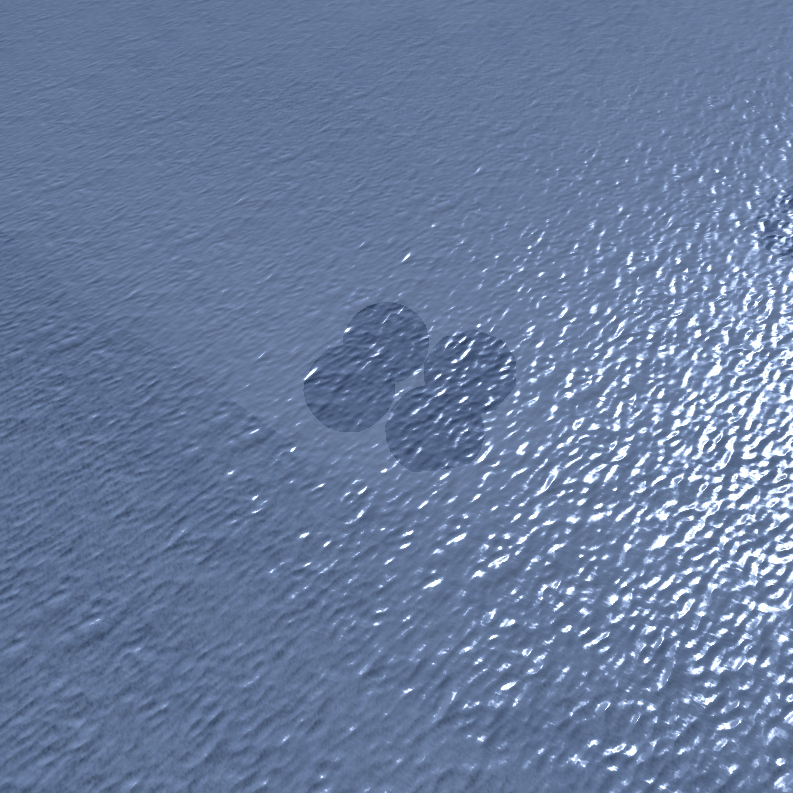
\includegraphics[width=0.9\linewidth]{images/waterWaves.jpg}
  \caption{The water.}
  \label{fig:waterWaves}
\end{subfigure}%
\begin{subfigure}{.5\textwidth}
  \centering
  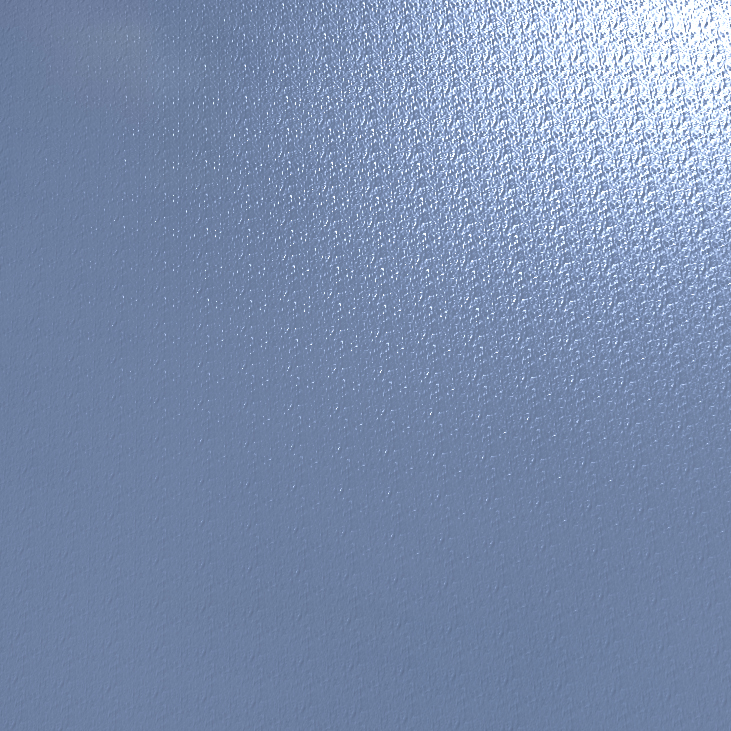
\includegraphics[width=0.9\linewidth]{images/waterGlimmer.jpg}
  \caption{Glittering water.}
  \label{fig:waterGlistering}
\end{subfigure}
\caption[Noise comparison]{\textit{Comparison of noise functions}}
\label{fig:water}
\end{figure}
Waves on the beaches is made by having several sinus waves aggregate horizontally to vary the wave fronts, and by having a sinus wave that control the vertical assent/decent of the waves. It is hard to catch on a screen shot, but an image of the waves in the world is shown in figure \ref{fig:waves}
\begin{figure}[H]
  \centering
  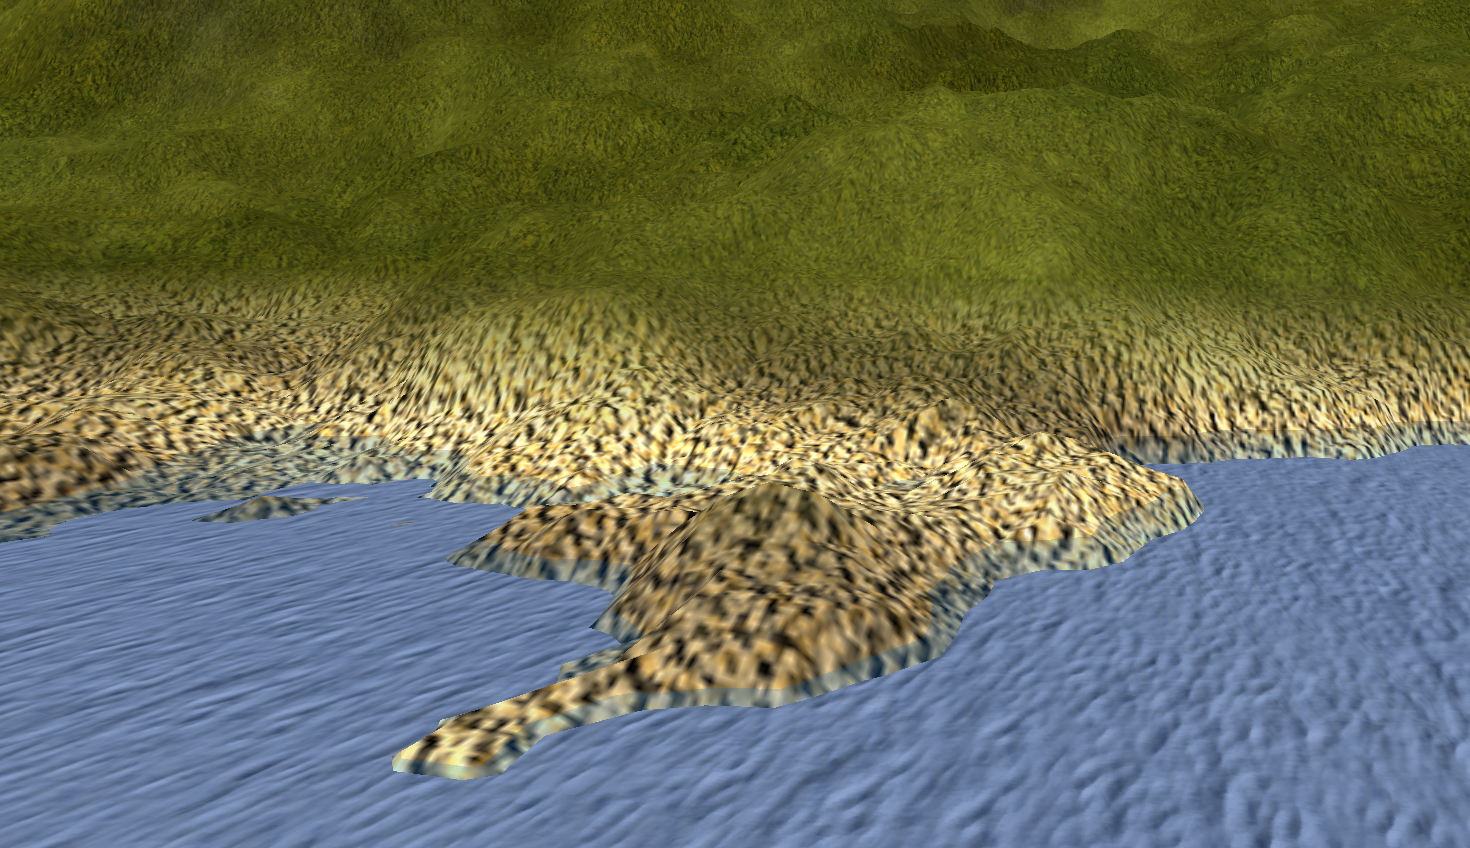
\includegraphics[width=0.9\linewidth]{images/waves.jpg}
  \caption{The waves are seen at the beach.}
  \label{fig:waves}
\end{figure}%
The sky is reflected in the water by using an image which is the projection of the sky onto the ocean as a texture for the water. This texture is moving with the camera in the xz-plane. An example is seen in figure \ref{fig:skyReflection}. It could be improved in the future by taking the height of the camera in consideration as well, or to continuously project the sky onto the water according to the camera position. Currently the camera height do not change the reflection, making it a bit unrealistic if moving up and down.
\begin{figure}[H]
  \centering
  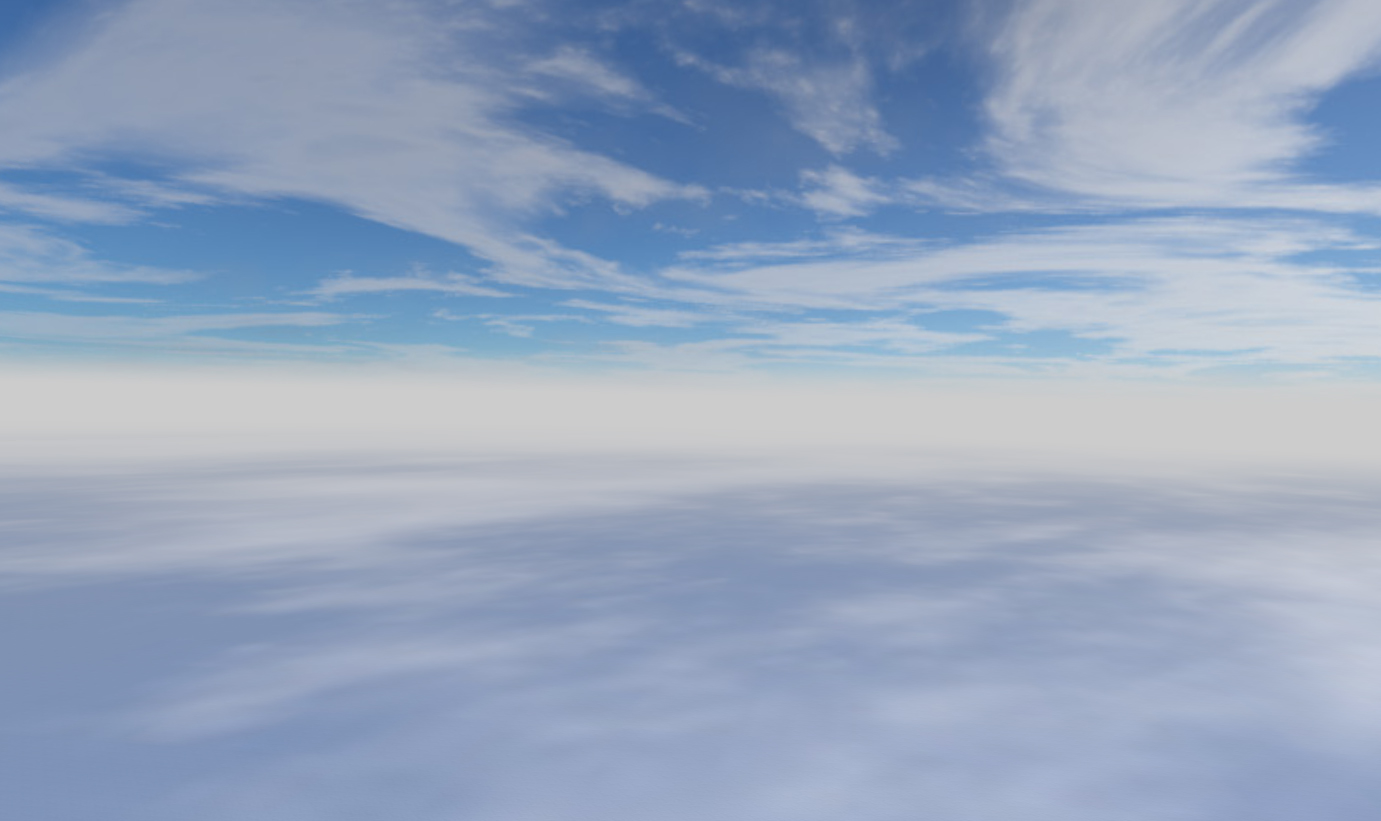
\includegraphics[width=0.9\linewidth]{images/reflectingSky.jpg}
  \caption{The sky reflected in the ocean.}
  \label{fig:skyReflection}
\end{figure}%

\newpage
\subsection{Terrain}
The terrain is generated by sampling a noise function and transforming its value into a height for each vertex. The noise in this case originates from a Simplex function. However, to get a realistically looking terrain it is not sufficient to sample this function only once for every vertex.

Fractional Brownian Motion is calculated by sampling the Simplex function at different frequencies and calculating a weighted sum over the samples \cite{FracBrownMotion}. The result is a nice looking height map. This allows for an arbitrary sample density. A few different sample densities are shown in figure \ref{fig:textureDensityComparison1}. A further possible extension would be to use tessellation, which would allow for a terrain with arbitrary fine details.  

\begin{figure}[H]
\begin{subfigure}{.5\textwidth}
  \centering
  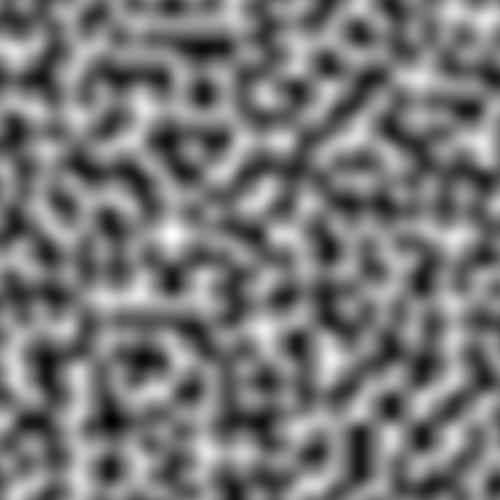
\includegraphics[width=0.9\linewidth]{images/Simplex.jpg}
  \caption{Height map generated from single-octave simplex noise}
  \label{fig:sub1}
\end{subfigure}%
\begin{subfigure}{.5\textwidth}
  \centering
  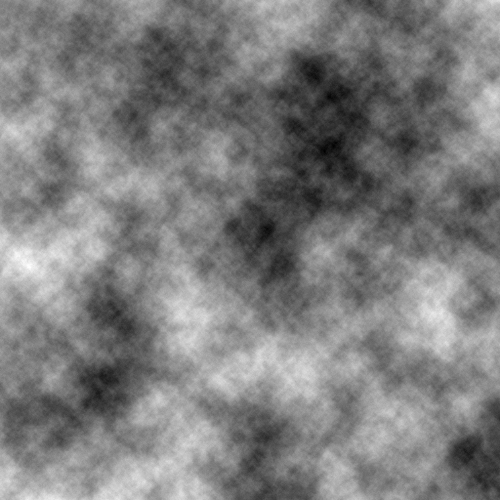
\includegraphics[width=0.9\linewidth]{images/FracBrownMotion.jpg}
  \caption{Height map generated with Fractional Brownian Motion}
  \label{fig:sub2}
\end{subfigure}
\caption[Noise comparison]{\textit{Comparison of noise functions}}
\label{fig:R_kitchen_example}
\end{figure}

The height map is finally assured to always slope into the ocean. This is done by first setting the all edge values to zero, then weighting the entire map with a thresholded Gaussian kernel, see figure \ref{fig:heightMapConstruction} below. 

\begin{figure}[H]
\begin{subfigure}{.32\textwidth}
  \centering
  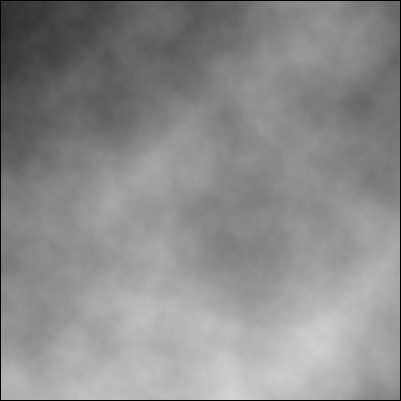
\includegraphics[width=0.9\linewidth]{images/heightMapRaw.jpg}
  \caption{Height map with edge set to zero.}
  \label{fig:heightMapRaw}
\end{subfigure}%
\begin{subfigure}{.32\textwidth}
  \centering
  
\includegraphics[width=0.9\linewidth]{images/heightMapKernel.jpg}
  \caption{Thresholded Gaussian kernel}
  \label{fig:heightMapKernel}
\end{subfigure}
\begin{subfigure}{.32\textwidth}
  \centering
  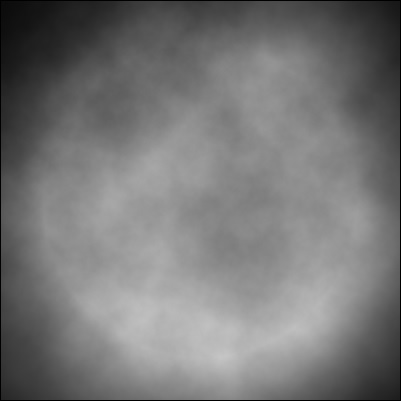
\includegraphics[width=0.9\linewidth]{images/heightMapFinal.jpg}
  \caption{Final height map.}
  \label{fig:heightMapFinal}
\end{subfigure}
\caption[Height map construction]{\textit{All steps in the creation of the height map.}}
\label{fig:heightMapConstruction}
\end{figure}

\begin{figure}[H]
\begin{subfigure}{.5\textwidth}
  \centering
  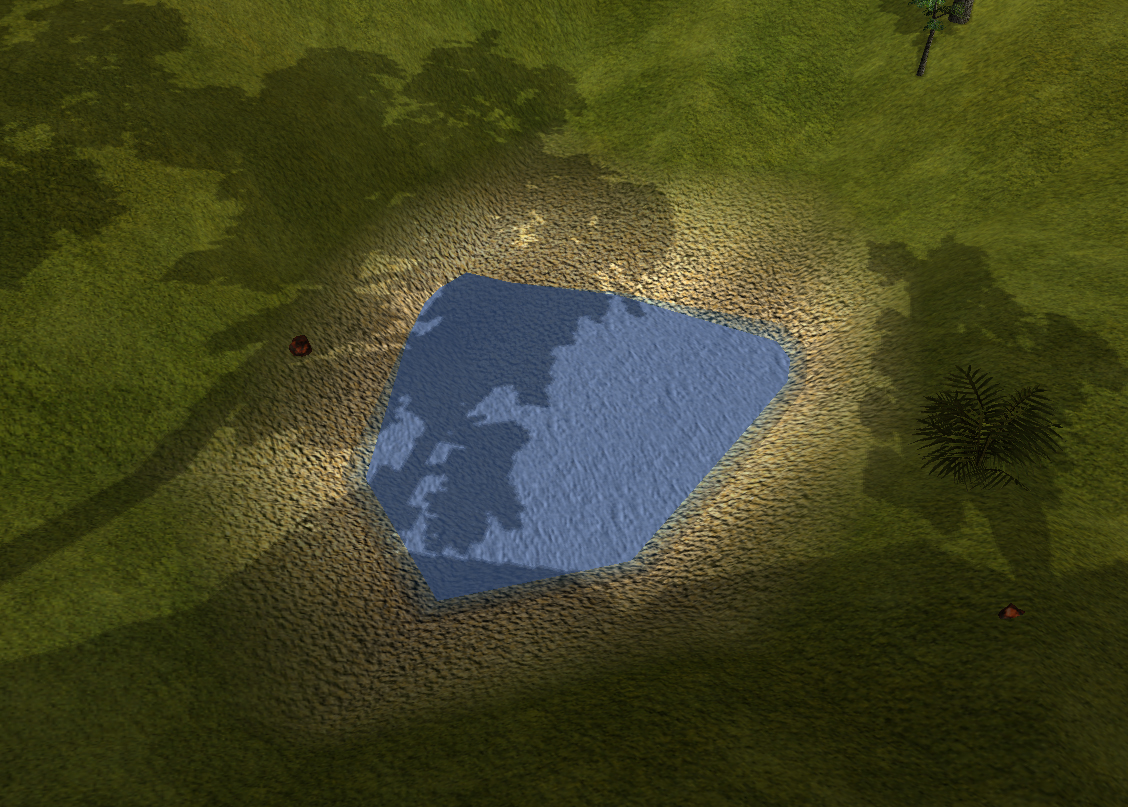
\includegraphics[width=0.9\linewidth]{images/terrainDensityComparison1_05.jpg}
  \caption{Density 0.5}
  \label{fig:textureDensity05}
\end{subfigure}%
\begin{subfigure}{.5\textwidth}
  \centering
  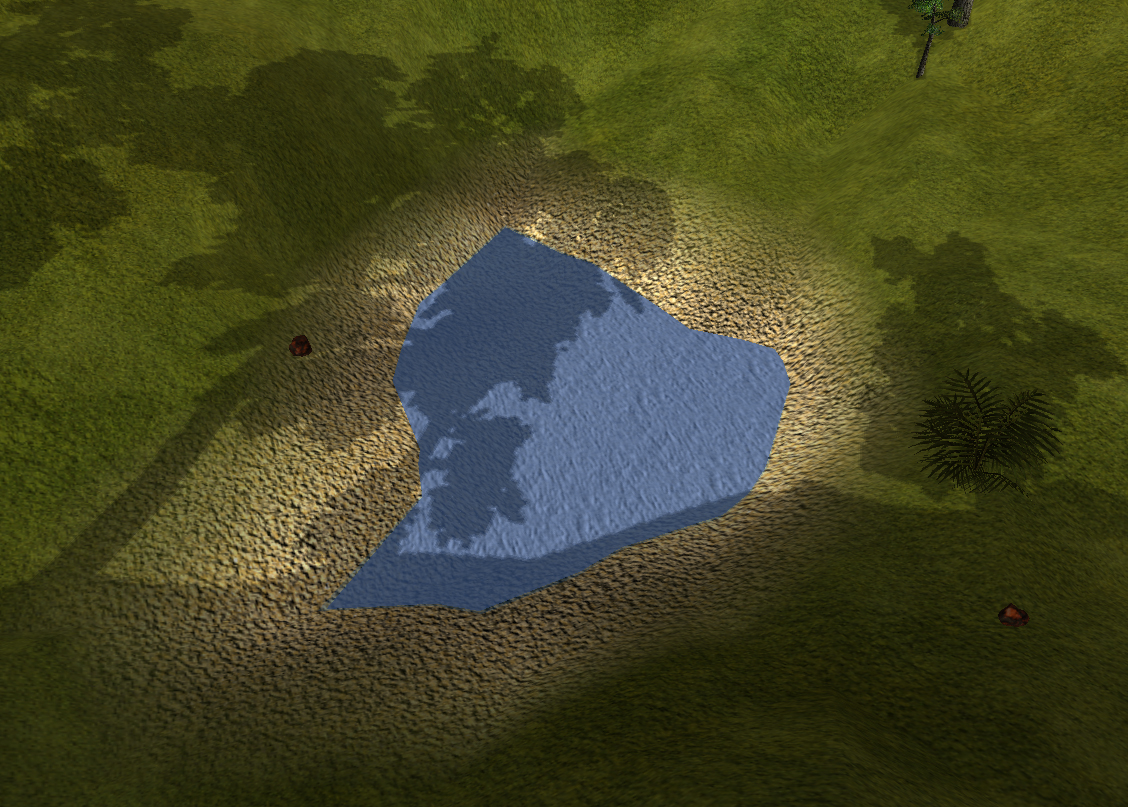
\includegraphics[width=0.9\linewidth]{images/terrainDensityComparison1_1.jpg}
  \caption{Density 1.0}
  \label{fig:textureDensity1}
\end{subfigure}%

\begin{subfigure}{.5\textwidth}
  \centering
  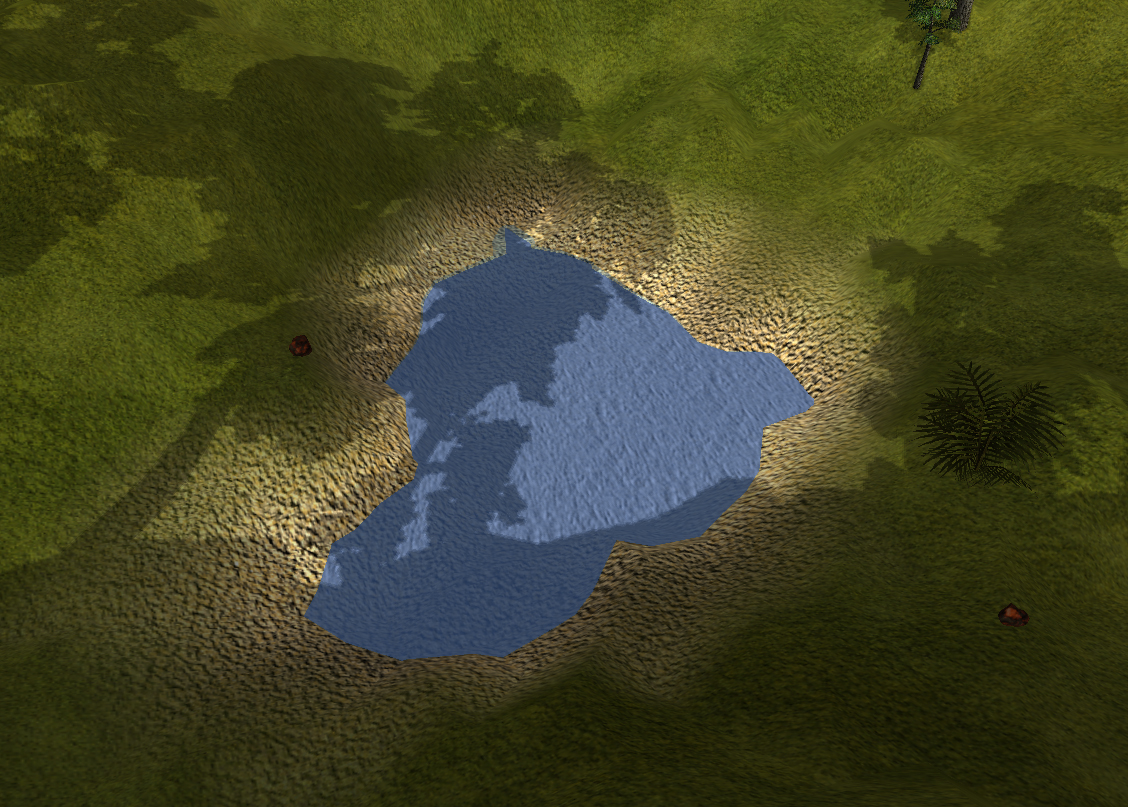
\includegraphics[width=0.9\linewidth]{images/terrainDensityComparison1_2.jpg}
  \caption{Density 2.0}
  \label{fig:textureDensity2}
\end{subfigure}%
\begin{subfigure}{.5\textwidth}
  \centering
  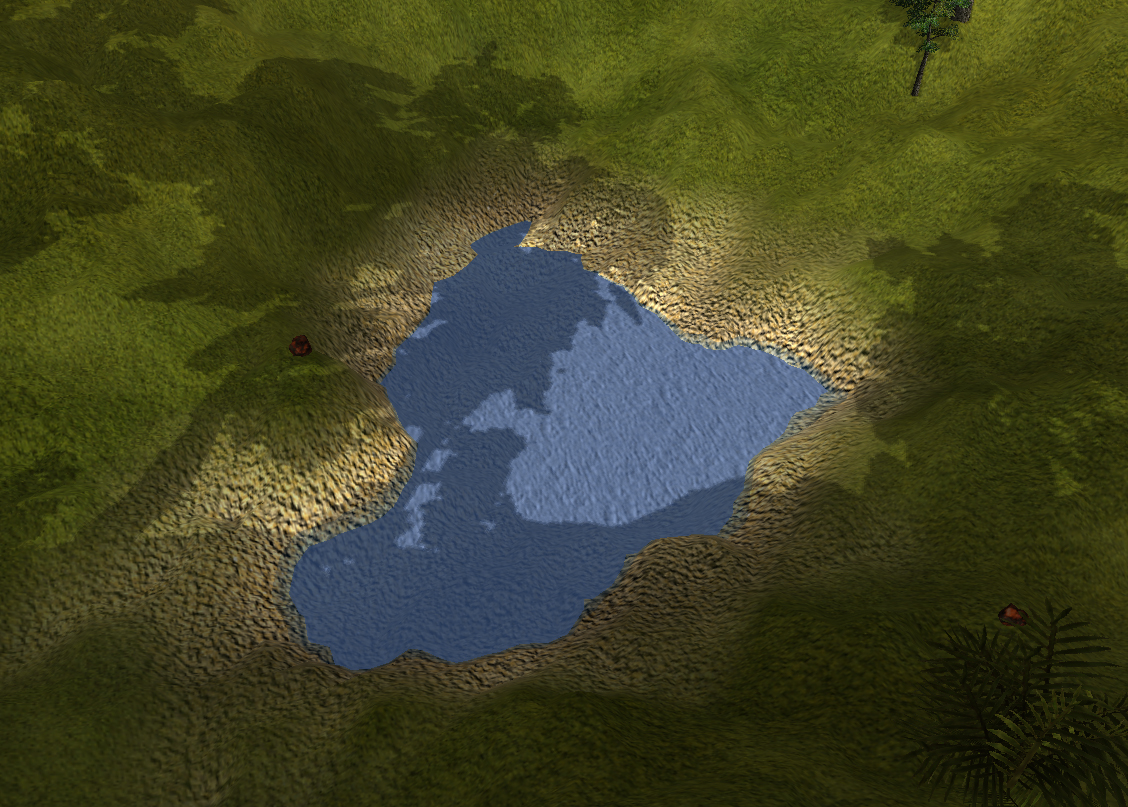
\includegraphics[width=0.9\linewidth]{images/terrainDensityComparison1_5.jpg}
  \caption{Density 5.0}
  \label{fig:textureDensity5}
\end{subfigure}%

\begin{subfigure}{.5\textwidth}
  \centering
  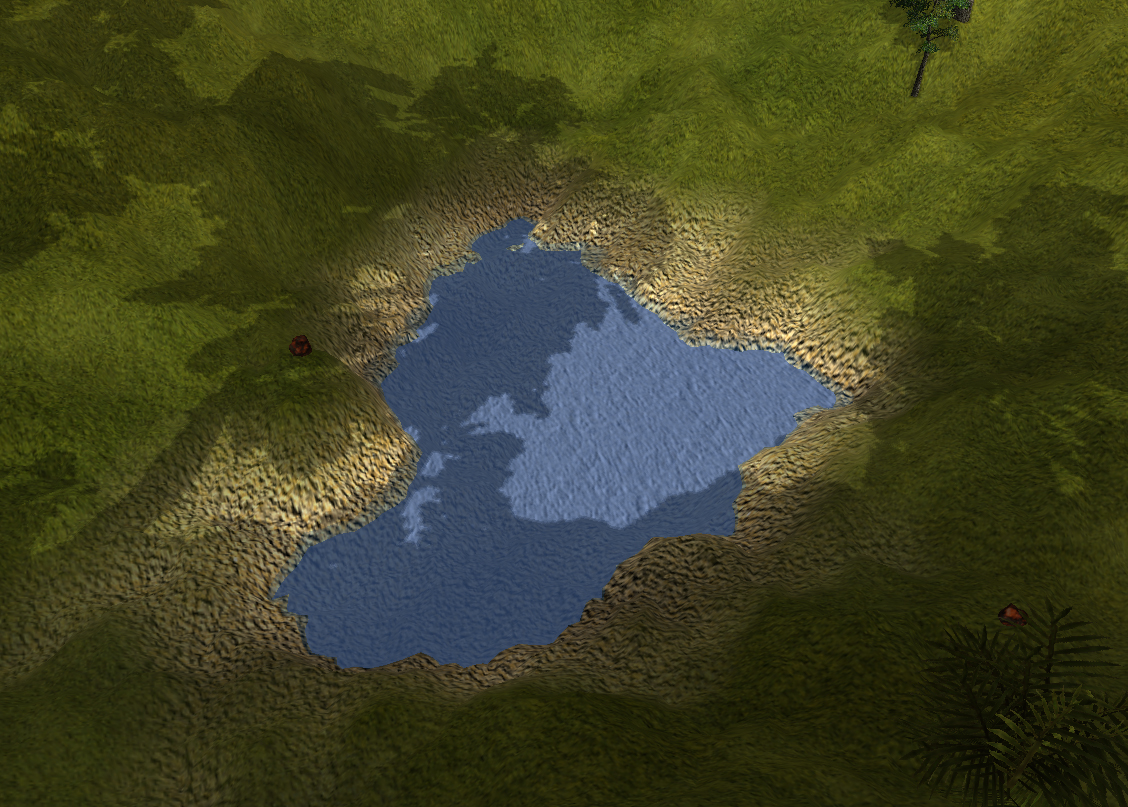
\includegraphics[width=0.9\linewidth]{images/terrainDensityComparison1_10.jpg}
  \caption{Density 10.0}
  \label{fig:textureDensity10}
\end{subfigure}%
\begin{subfigure}{.5\textwidth}
  \centering
  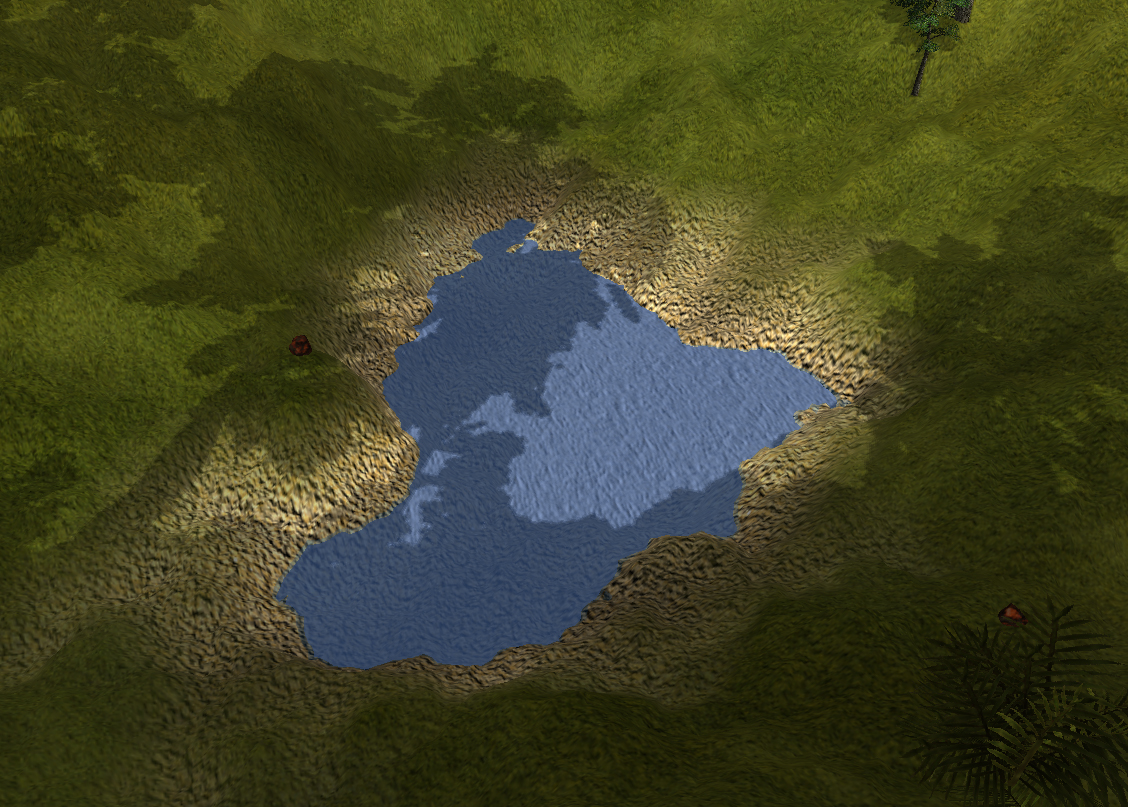
\includegraphics[width=0.9\linewidth]{images/terrainDensityComparison1_15.jpg}
  \caption{Density 15.0}
  \label{fig:textureDensity15}
\end{subfigure}%
  \caption{A comparison of different vertex and sample density, from 0.5 to 15 vertexes per OpenGL length units. Waves are shown in some of the images, as the wave generator currently doesn't distinguish between lakes and oceans.}
  \label{fig:textureDensityComparison1}
\end{figure}

\newpage
\subsection{Ground}
The ground is textured using a non-linear multi-texturing approach based on both altitude and terrain slope. Currently only three textures are used: one sandy, one grassy and one rocky, which can be seen in figure \ref{fig:textures}.

\begin{figure}[H]
\begin{subfigure}{.32\textwidth}
  \centering
  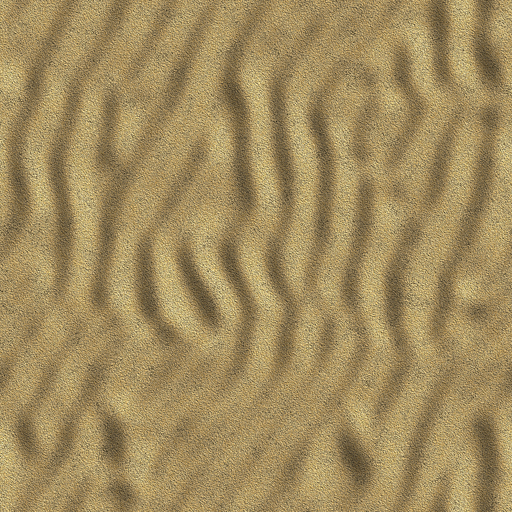
\includegraphics[width=0.9\linewidth]{images/textureSand.jpg}
  \caption{The sand/beach texture.}
  \label{fig:textureSand}
\end{subfigure}%
\begin{subfigure}{.32\textwidth}
  \centering
  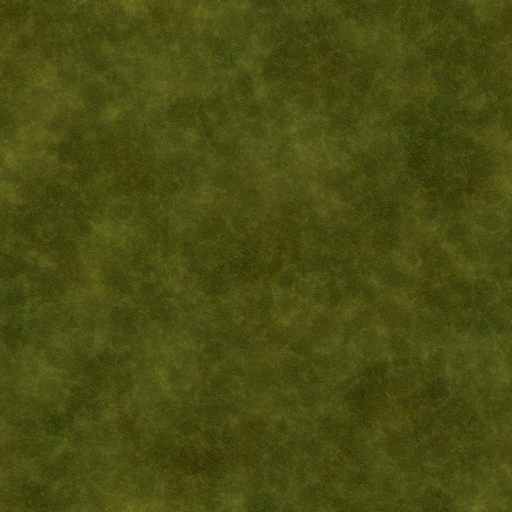
\includegraphics[width=0.9\linewidth]{images/textureGrass.jpg}
  \caption{The grass/ground texture.}
  \label{fig:textureGrass}
\end{subfigure}
\begin{subfigure}{.32\textwidth}
  \centering
  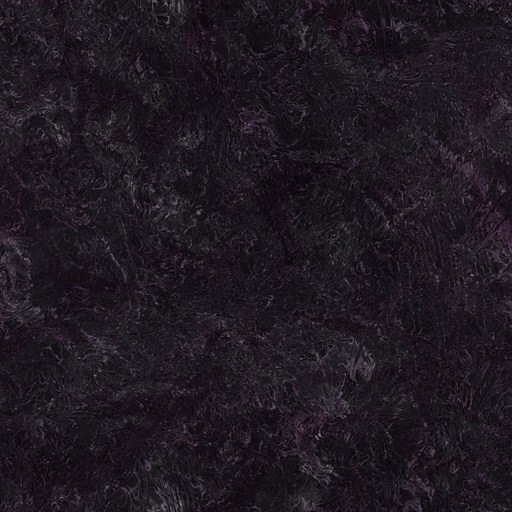
\includegraphics[width=0.9\linewidth]{images/textureRock.jpg}
  \caption{The rock/volcano texture.}
  \label{fig:textureRock}
\end{subfigure}
\caption[Ground textures]{\textit{Textures used for the ground.}}
\label{fig:textures}
\end{figure}

The texture blending allows for the mountain to reach almost down to the ocean while still letting the fields and the highland being very grassy. The blending between rock and grass make the landscape more alive and less dull. In figure \ref{fig:textureComparison1} and \ref{fig:textureComparison2} a simple blending using linear interpolation between rock and grass is compared to our more advanced method. In our method the interpolation between the different textures vary between being squared, linear and square-root, depending on the slope and altitude.
\begin{figure}[H]
\begin{subfigure}{0.9\textwidth}
  \centering
  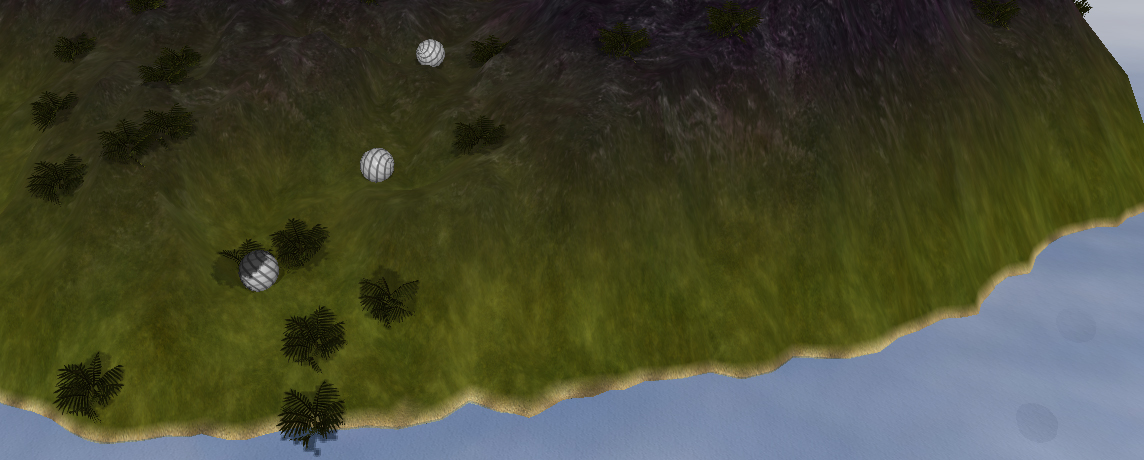
\includegraphics[width=0.9\linewidth]{images/textureBlendingComparison1_simple.jpg}
  \caption{Simple linear interpolation.}
\end{subfigure}%

\begin{subfigure}{0.9\textwidth}
  \centering
  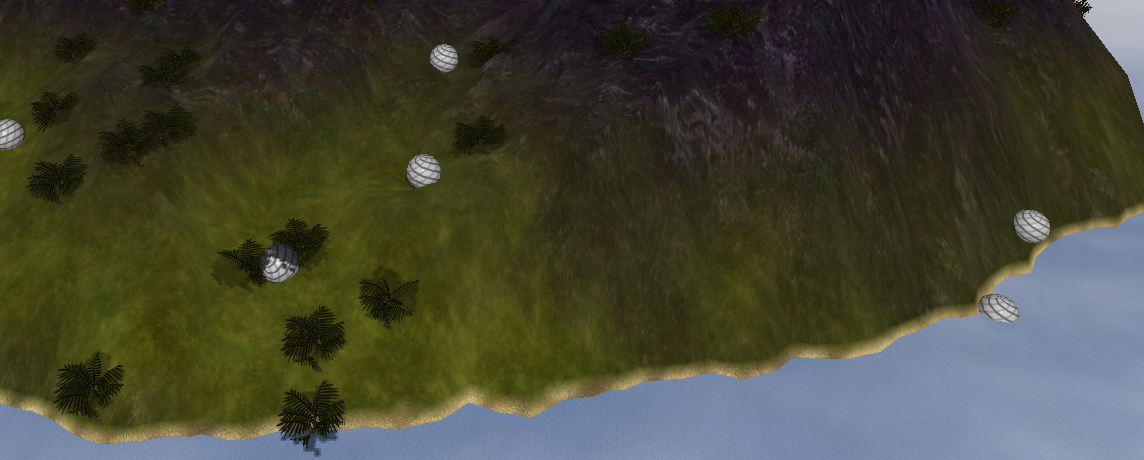
\includegraphics[width=0.9\linewidth]{images/textureBlendingComparison1_advanced.jpg}
  \caption{Advanced non-linear texture blending.}
\end{subfigure}%
\label{fig:textureComparison1}
\caption{A comparison between a simple interpolation of the textures (a) and our method (b). Notice the varying tone of the grass as well as the deep mountain slope to the right in (b).}
\end{figure}

\newpage
\begin{figure}[H]
\begin{subfigure}{0.9\textwidth}
  \centering
  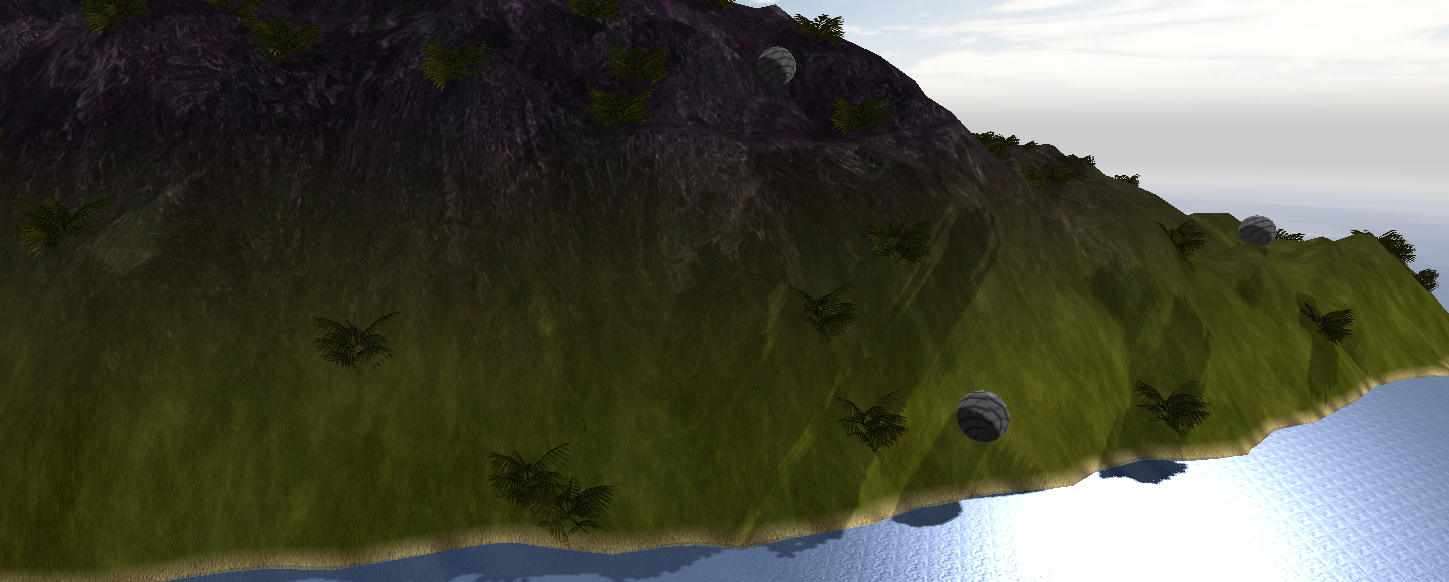
\includegraphics[width=0.9\linewidth]{images/textureBlendingComparison2_simple.jpg}
  \caption{Simple linear interpolation.}
\end{subfigure}

\begin{subfigure}{0.9\textwidth}
  \centering
  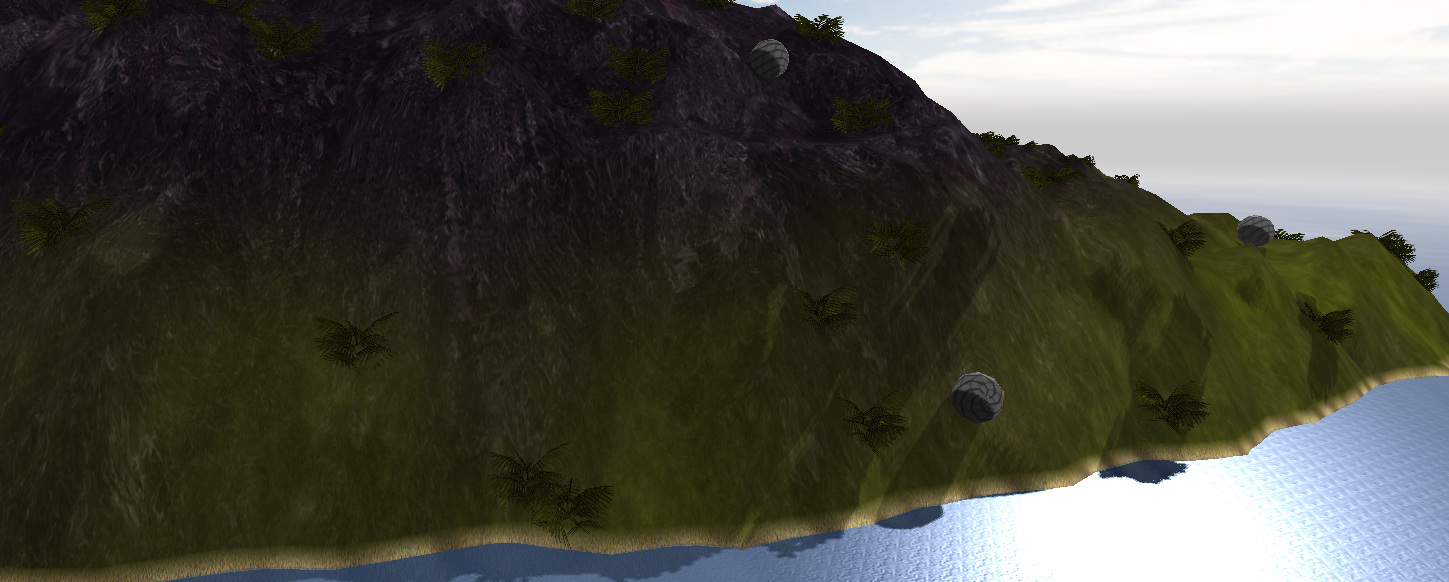
\includegraphics[width=0.9\linewidth]{images/textureBlendingComparison2_advanced.jpg}
  \caption{Advanced non-linear texture blending.}
\end{subfigure}
\label{fig:textureComparison2}
\caption{A comparison between a simple interpolation of the textures (a) and our method (b). Notice the varying tone of the grass as well as the much greener upper region to the right in (b).}
\end{figure}

\newpage
\subsection{Vegetation}
In order for the world to be more interesting than just an island in the middle of the sea, it needs some additional objects aswell, thus plants are placed using two slightly different approaches.

First a base layer of smaller bushes are placed uniformly over the landmass, with a randomized orientation and scaling. Then a few points are designated as forest centers, around these trees are placed using a Gaussian distribution, again the trees have some scale and rotation randomly selected.
TODO: Bildexempel på skogar? (ev)

Placing the objects is done by generating a coordinate, and checking it for suitability, for example nothing can be placed in the water, or to far up on a mountain/volcano.

TODO Häger: Berätta om de olika växterna (vilka använder vi, hur många olika texturer vi använder. hur de är uppbyggda. Hur texturerna måste vara för att alpha mip-mapping ska fungera). Bild-exempel?

TODO Häger: exempelbild på när vår alpha-mip-mapping inte riktigt räcker till?  (Att vi nästan inte ser några fel (förutom grått på håll, vilket kan misstas för distance-fog).

\newpage
\begin{figure}[H]
\begin{subfigure}{0.9\textwidth}
  \centering
  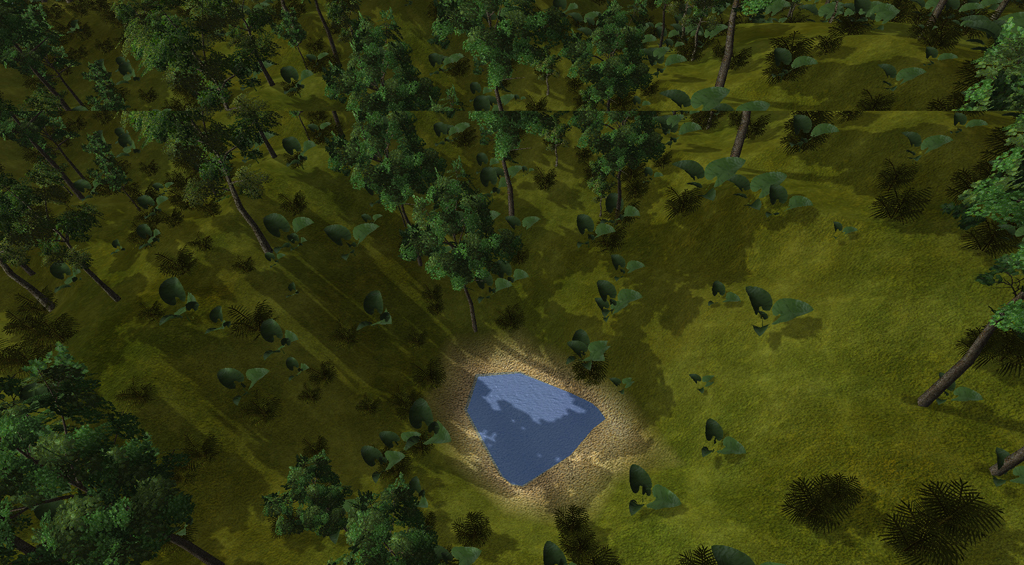
\includegraphics[width=0.9\linewidth]{images/content1.jpg}
  \caption{A small water hole in the middle of the forest at the late afternoon.}
  \label{fig:vegetation0}
\end{subfigure}%
\\
\begin{subfigure}{0.9\textwidth}
  \centering
  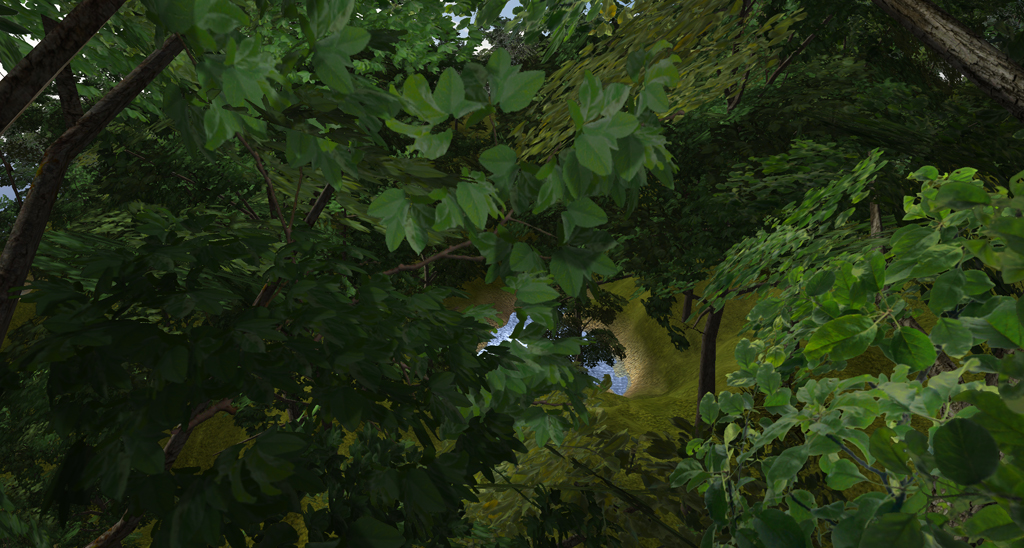
\includegraphics[width=0.9\linewidth]{images/vegetation1.jpg}
  \caption{The same water hole seen in (a), but perceived through the vegetation.}
  \label{fig:vegetation1}
\end{subfigure}%
\\
\begin{subfigure}{0.9\textwidth}
  \centering
  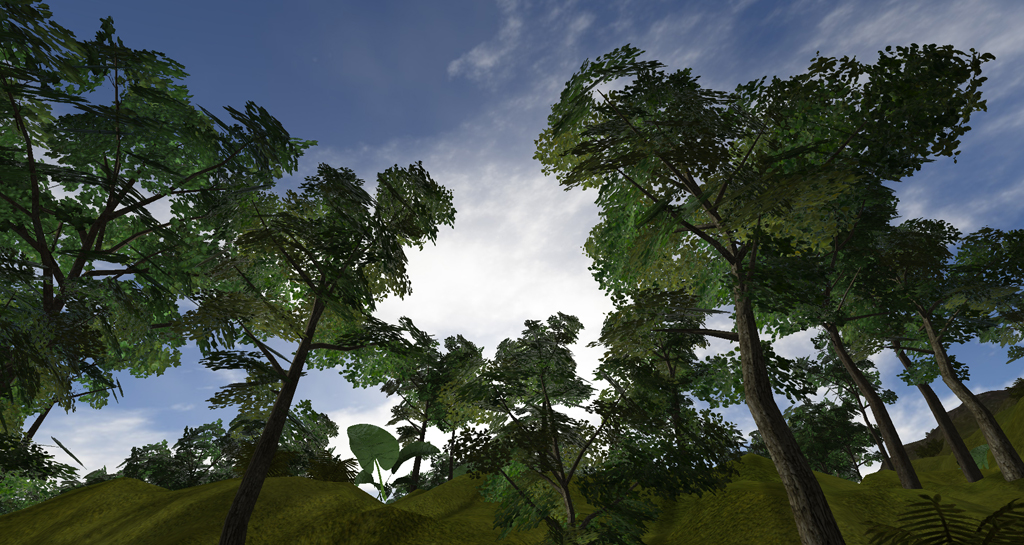
\includegraphics[width=0.9\linewidth]{images/vegetation2.jpg}
  \caption{Trees in the outskirt of a forest, portrayed against the sun.}
  \label{fig:vegetation2}
\end{subfigure}
\label{fig:vegetationViwes}
\end{figure}

\newpage
\subsection{Volcano}
The volcano generator changes the terrain on a spot to that of a volcano, such as the one seen in figure \ref{fig:volcano1}.
\begin{figure}[H]
  \centering
  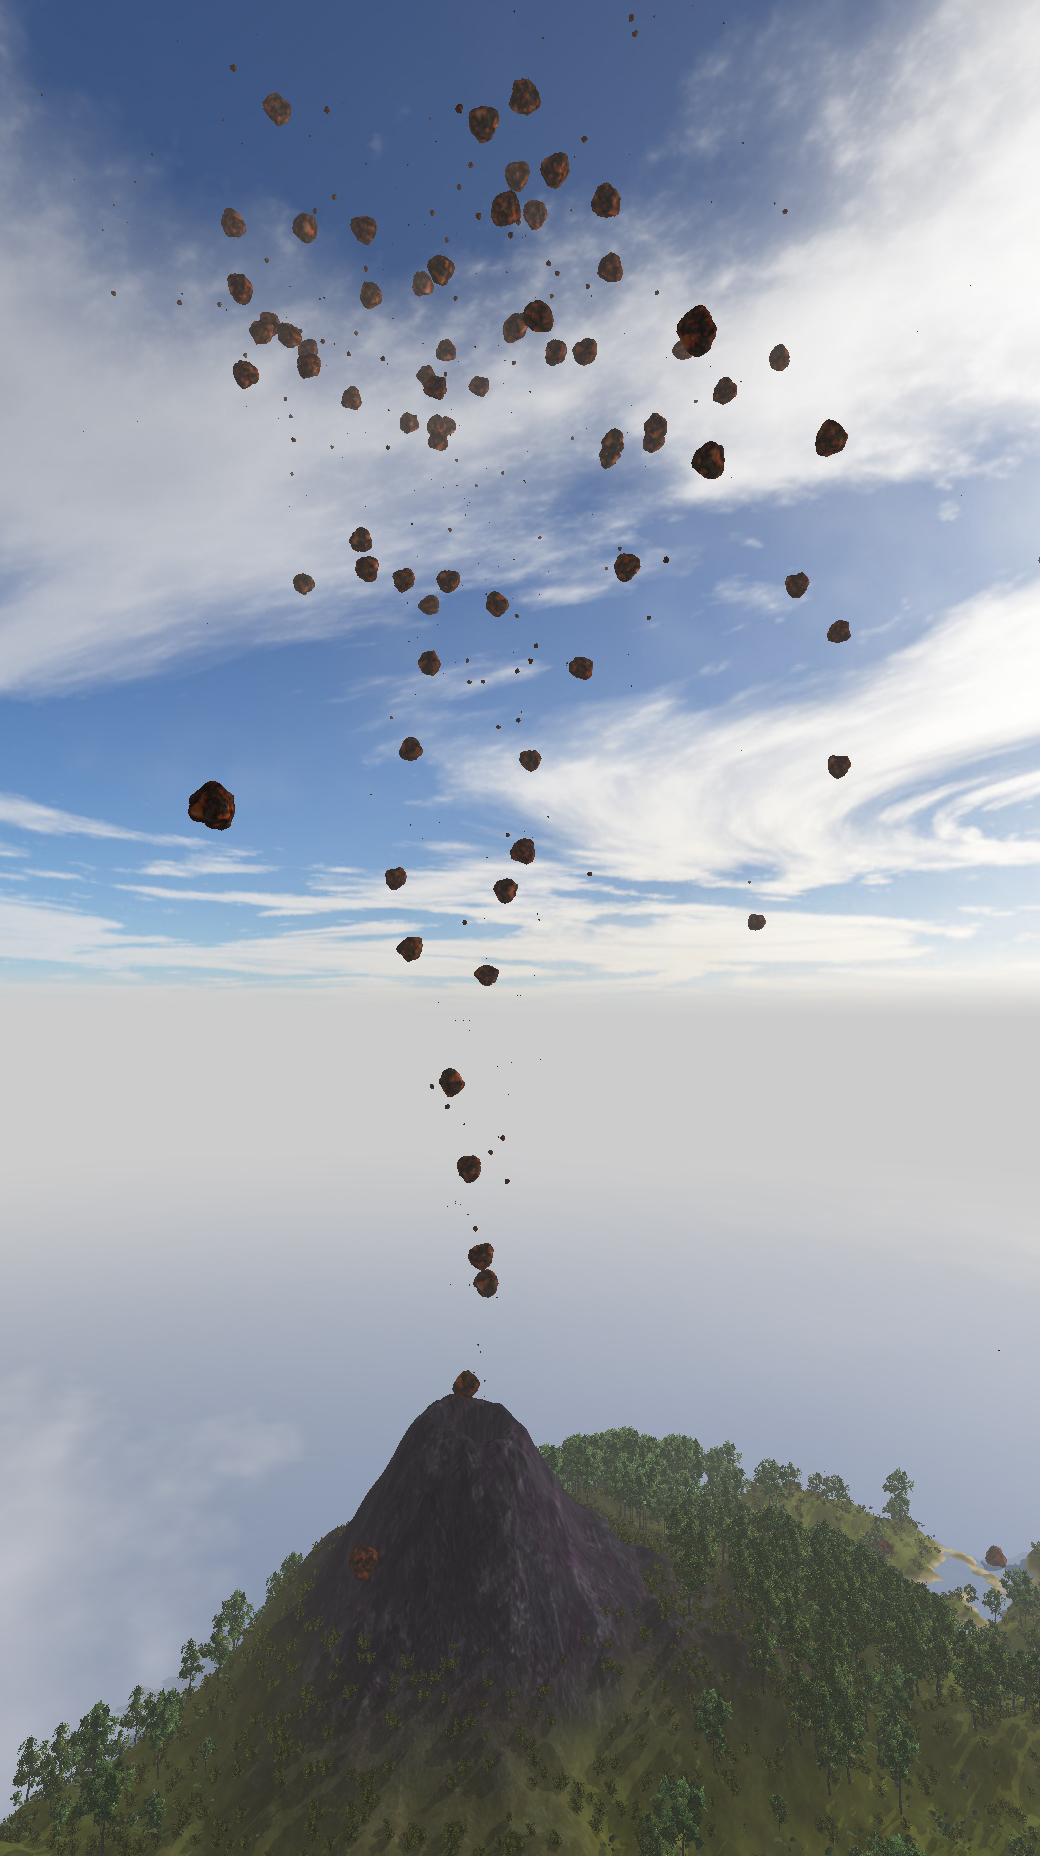
\includegraphics[width=0.7\linewidth]{images/volcano.jpg}
  \caption{A vulcano.}
  \label{fig:volcano1}
\end{figure}%
\newpage
The volcano is made from one addition of a 2D-Gaussian to the terrain, and of a subtraction of a smaller 2D-Gaussian which creates the eruption hole. It erupts and spews out lava stones as a particle effect. Currently only one volcano is generated on each island, and it is placed on the highest point on the terrain.

Lava stones are made up of 5 different stone models of different sizes. They have full 3D sphere physics, including collision with each other and the terrain. Lava stones are created in the eruption hole with a randomized linear and angular momentum, forcing them to burst out of the volcano in a spraying fashion. When the lava stones enter water and sink too deep, they are re-spawned in the volcano and sent out though the hole again.

The physics can be reversed in time, making the stones return to the volcano hole. When they enter the volcano they are placed where they were when they disappeared into the water last, with all the physical properties reset to how they were at that time as well. This makes lava stones come up through the water and moving in a reversed trajectory into the volcano, repeating the feat over and over, and providing a nice visual for the audience.

\begin{figure}[H]
  \centering
  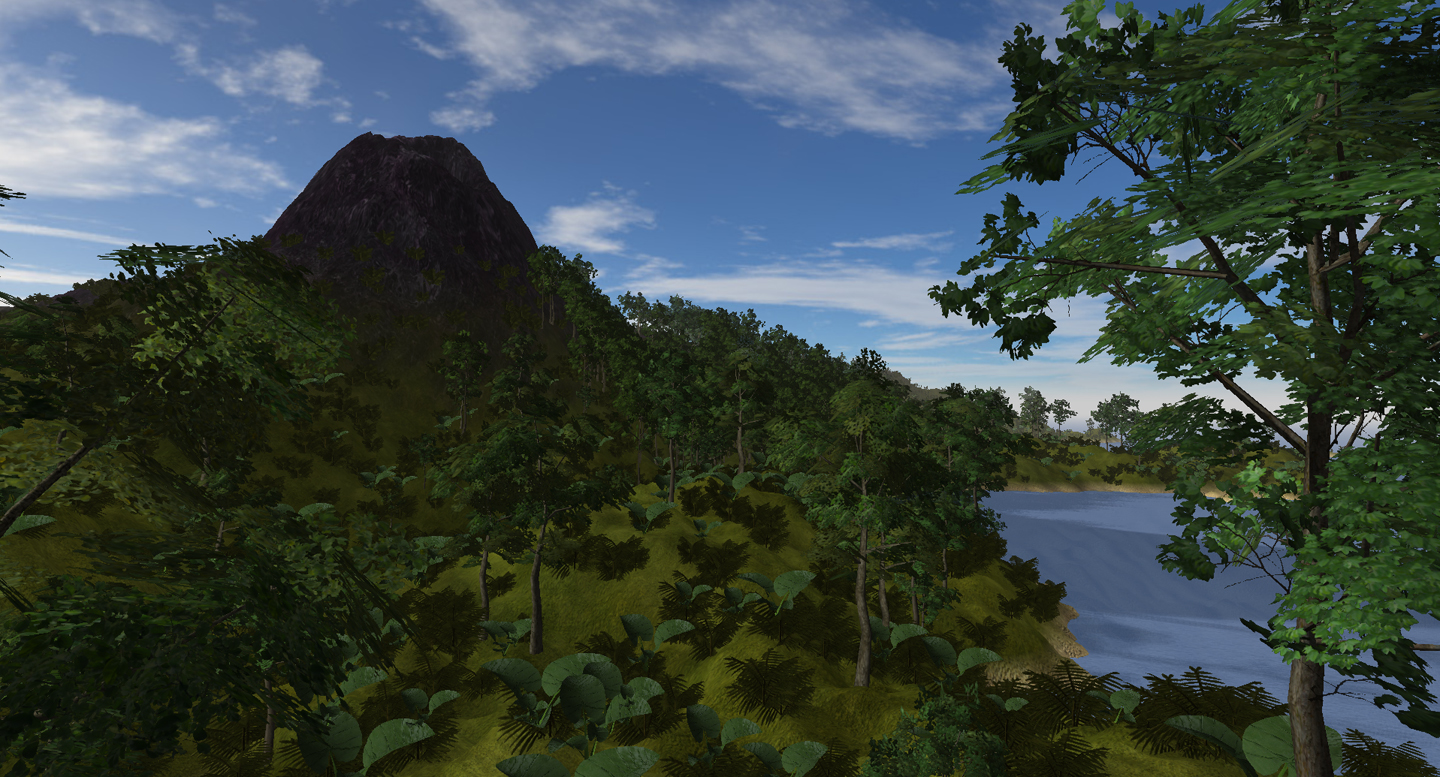
\includegraphics[width=0.9\linewidth]{images/volcano3.jpg}
  \caption{A (currently) dormant volcano and its surrounding.}
  \label{fig:vulcano2}
\end{figure}%

A typical volcano and its surroundings is seen in figure \ref{fig:volcano2}. In figure \ref{volcanoEruptions} other views of the lava stone particle effect is shown.

\newpage
\begin{figure}[H]
\begin{subfigure}{\textwidth}
  \centering
  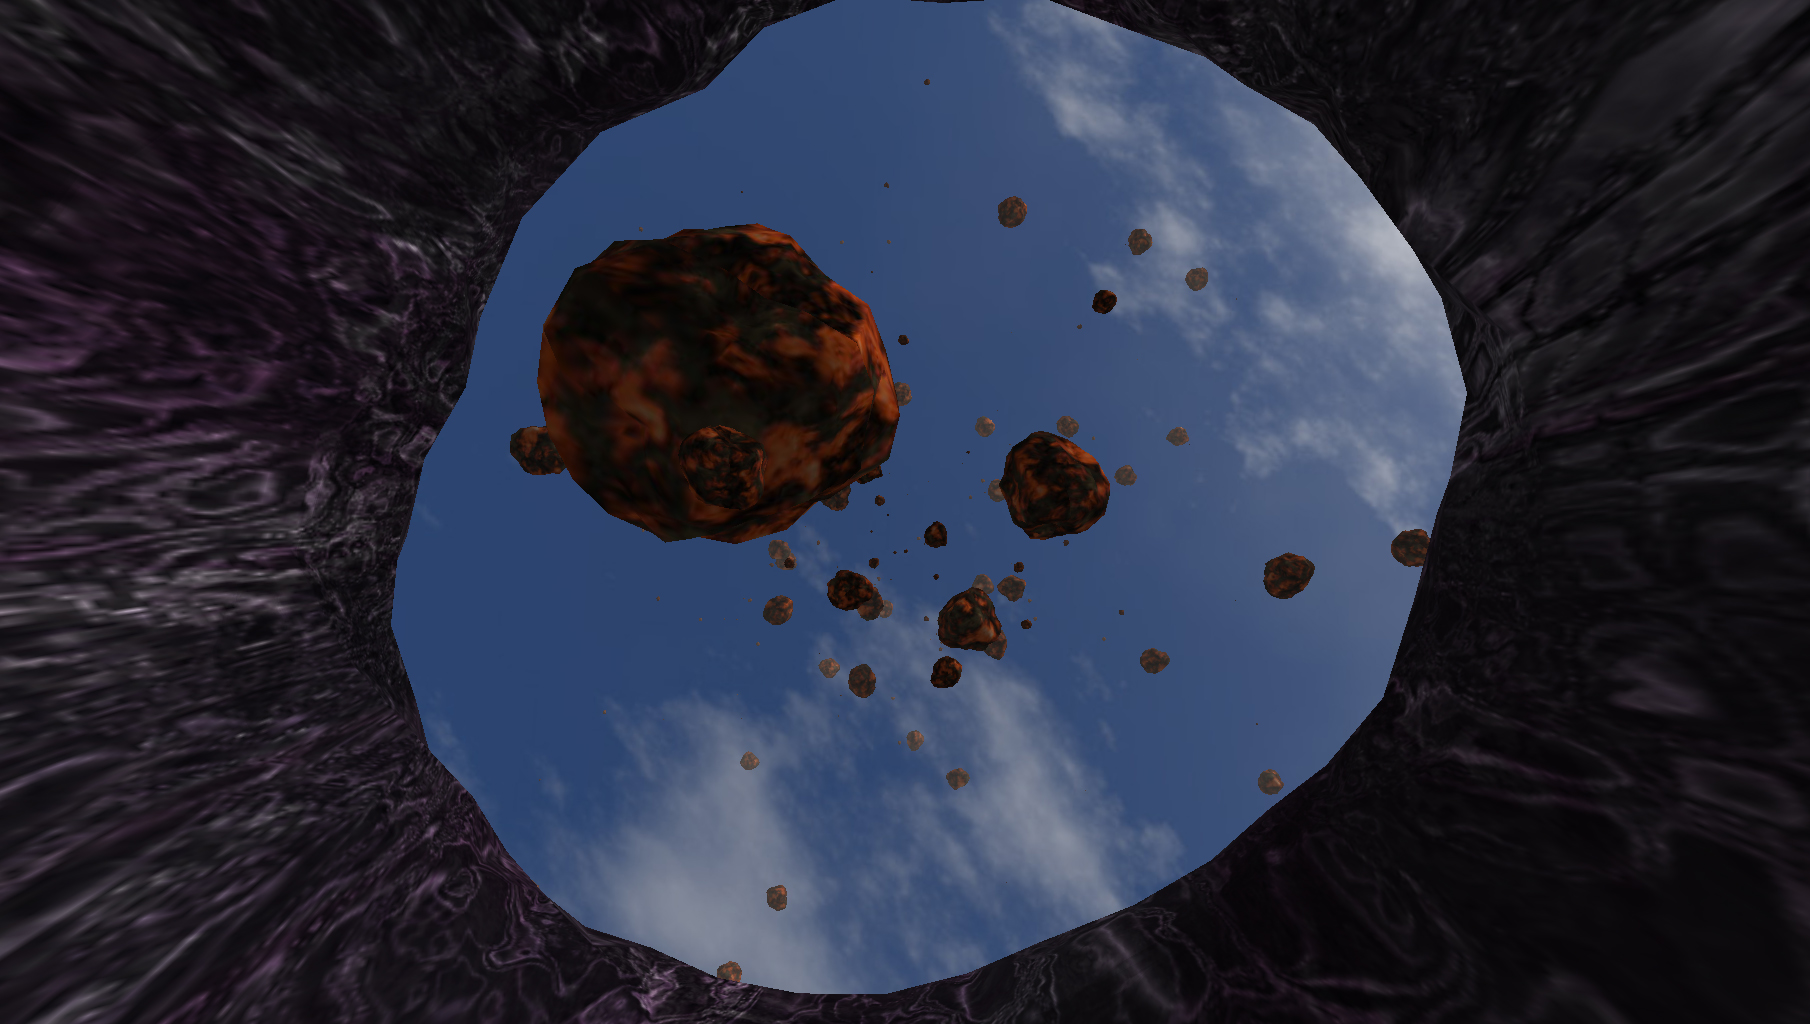
\includegraphics[width=0.9\linewidth]{images/Volcano1.jpg}
  \caption{A Volcano eruption seen from inside the volcano)}
  \label{fig:volcanoEruption1}
\end{subfigure}%

\begin{subfigure}{\textwidth}
  \centering
  \includegraphics[width=0.9\linewidth]{images/Volcano2.jpg}
  \caption{Volcano eruption on a small island seen from above.}
  \label{fig:volcanoEruption2}
\end{subfigure}
\caption[Noise comparison]{\textit{Volcano eruption, seen from different angles.}}
\label{fig:volcanoEruptions}
\end{figure}



